%
% CS 259 - Winter 2013
% Formal Modeling and Analysis of the Bluetooth 4.0 Pairing Protocol
% David (Wei) Jia and Richard Hsu
% Stanford University
% 
% Requirements:
% + This file requires the acm_proc_article-sp.cls style file.
% + This file requires a cs259-bluetooth.bib file for the references.
% 

\documentclass{acm_proc_article-sp}
\usepackage{url} 
\usepackage{enumerate}
\usepackage{comment}

\begin{document}

% === Document Meta Data
\title{Formal Modeling and Analysis of \\ Bluetooth 4.0 Pairing Protocol}
\numberofauthors{2} 
\author{
    \alignauthor David (Wei) Jia \\
		\affaddr{Stanford University} \\
	    \email{djia@stanford.edu}
	\alignauthor Richard Hsu \\
	    \affaddr{Stanford University} \\
	    \email{rhsu@cs.stanford.edu}
}

% === Title Display of Information
\maketitle

% === Abstract
\begin{abstract}
Bluetooth is a wireless technology for exchanging data over short distances and is built into many of the devices used in daily life such as smartphones and laptops. Bluetooth allows communication between paird devices. The pairing is done through Bluetooth's pairing protocol known as Secure Simple Pairing (SSP) which has been established since Bluetooth 2.1+. Bluetooth security is important because sensitive and confidential information such as phone conversations, messages, and key strokes on a keyboard are often communicated through a pairing. We employ a formal model checker to verify the security properties of the pairing protocol used in Bluetooth 4.0, the latest iteration of the protocol. Using our formal Murphi model, we demonstrate and confirm previously known attacks on Bluetooth that have not yet been formalized. We then discuss a new attack found by our model as well as its implications to Bluetooth 4.0 security. Finally, we discuss and recommend possible fixes that could be employed to avoid the attacks we have found. Through this formal modeling we expand on the security verification of Bluetooth pairing protocol.
\end{abstract}


% === Introduction
\section{Introduction}

Bluetooth is a wireless technology that is ubiquitous in many modern applications. Users rely on it to transfer data between smartphones, laptops, on-board car systems, and headsets. Bluetooth technology also exists in more peripheral items such as printers, mice, keyboards, and speakers. Because Bluetooth serves as an underlying systems for so many communication systems that are used on a daily basis, senstivie and confidential information can often times be passed through the supposedly secure paired channel. For example, a security breach on Bluetooth could potentially lead to eavesdropping on phone conversations and keylogging password entries. Thus, we analyze Bluetooth in this paper through a formal modeling and analysis in hopes of shedding light on its security.

In this paper, we focus our attentions on the Bluetooth 4.0 Protocol \cite{bluetooth:sig4}, which is the most recent version of the technology at the time of writing.


% === Bluetooth Overview
\section{Bluetooth Overview}
Bluetooth is a wireless technology standard used for exchanging data over a short distance. It utilizes short-wavelength radio transmission and is implemented in devices ranging from hands-free headsets to computer peripherals such as a mouse or keyboard. These devices are fairly ubiquitous today. Some examples of the data transferred between devices via Bluetooth include inputs from a wireless keyboard, contacts transferred between phones, files transferred between computers, and even patient health data from medical sensors to servers. Each Bluetooth responder device (such as a laptop) can be paired with up to seven Bluetooth initiator devies (such as a keyboard or mouse).

Because of the wide range in the application of Bluetooth, the security of the Bluetooth communication is vitally important. The major part of Bluetooth that becomes vulnerable to attackers is the the pairing protocol when two or more devices first initiate connections with one another. The connection process creates a personal area network and requires authentication and encryption to remain secure. Since Bluetooth 2.1, Secure Simple Pairing (SSP) \cite{bluetooth:sig2} has been implemented and further improved in subsequent versions leading to the current version of Bluetooth 4.0 discussed in the current paper.

\subsection{Secure Simple Pairing Protocol}

Bluetooth 4.0 Secure Simple Pairing contains four main association models depending on the devices involved:
\begin{enumerate}[1.]
    \item{Just Works (JW)} When at least one device does not have display nor input channel. Example: wireless headset.
    \item{Numeric Comparison (NC)} When both devices have a display and at least one has a binary input channel for a yes or no response. Example: pairing between smartphones.
    \item{Passkey Entry (PE)} When one device has an input channel but no display and the other device has a display but no input channel. Example: Wireless keyboard.
    \item{Out of Band (OoB)} When both devices support a common additional wireless or wired communication technology for purpose of device discovery or cryptographic channels. Example: Near Field Communication (NFC).
\end{enumerate}

The SSP protocol is completed in five phases. SSP follows the same steps in these five phases for all four association models with the exception of phase 2. The process of pairing through the five phases is described in detail below:

In our analysis, we will only consider the JW and NC models since the PE model is just a special case of the NC model and OoB's security is dependent on the security of an out of band cryptographic channel.

\subsubsection{Phase 1: Public Key Exchange}
In this phase, Elliptic Curve Diffie-Hellamn (ECDH) key exchange \cite{mingard} is completed by the initiating (Device A) and non-initiating, or responding device (Device B). Both devices generate a public-private key pair using ECDH. The public key of each device is sent to the other device. Note that according to the official Bluetooth Specifications, this key pair do not need to be generated at each time a pairing occurs. Each device may discard its key pair and generate a new one at any time, but this is not a requirement.

\subsubsection{Phase 2: Authentication Stage 1}
In this stage, each of the four associated models has a different, but relatively similar authentication process. In each of the associated models, both devices generate a random nonce, $N_a$ and $N_b$, respectively for Device A and Device B. Device B, the non-initiating device then computes a commitment value $C_b = f_1(PK_b, PK_a, N_b, 0)$, where $PK_a$ is the public key for Device A and $PK_b$ is the public key for Device B, and $f_1$ is SHA256 dependent one-way hash-function that generates a 128-bit value with the given input.

After $C_b$ is generated, it along with $N_b$ is sent to Device A. Device A also sends $N_a$ to Device B. Next, Device A computes the same commitment value $C_a = f_1(PK_b, PK_a, N_b, 0)$ and compares it with $C_b$. If they do not equal, then the pairing process is aborted. If they are equal, then the process proceeds, and diverges for each of the four associated models as follows until the end of Phase 2.

\begin{enumerate}[1.]
    \item{Just Works (JW)} In this associated model, since one of the devices can neither display nor input values, Phase 2 ends here and moves on to Phase 3.
    \item{Numeric Comparison (NC)} In this associated model, Phase 2 goes on to generate two verification codes to be displayed by the user. Each device $x$ generates a six-digit verification code $V_x = g(PK_a, PK_b, N_a, N_b)$, and displays it to the user. The user can then determine if $V_a = V_b$ and confirm the pairing and moves on to Phase 3.
    \item{Passkey Entry (PE)} In PE, the two devices decide upon a secret value, created by the users of the devices. If we are pairing two devices that both do not have screens, then the values are agreed upon by the user. If one device has a display, then the device generates a random value, which is shown on the device's display to be inputted into the other (input) device. This shared secret is turned into an $n$-bit number ($n$ depends on the length of the shared secret). Let the $i$-th bit for device $x$ be denoted as $r_{x_i}$. Since the secret is shared, the assumption is that all $r_{a_i} = r_{b_i}$ for all $i$. Then for each $i$, a commitment value, $C_{x_i} = f_1(PK_b, PK_a, N_{x_i}, r_{x_i})$ is generated for device $x$. The twenty commitment values are sent to the other device and compared. If any commitment values do not equal, then we abort the process. Otherwise, we move on to Phase 3.
    \item{Out of Band (OoB)} In OoB, after the commitment stage described completes, a shared secret comparison is done similar to the PE mode, except the external communication is complete through an external channel such as NFC.
\end{enumerate}

\subsubsection{Phase 3: Authentication Stage 2}
Phase 3 confirms that both devices have successfully completed the exchange during pairing. Device A generates exchange codes $E_a = f_3(DHKey, N_a, N_b, r_b, IOcapA, A, B)$ and Device B generates $E_b = f_3(DHKey, N_b, N_a, r_a, IOcapB, B, A)$, where $DHKey$ is the Diffie-Hellman key created in Phase 1. Both are sent to the other device. Each device then computes the exchange code for the other device and verifies that it is the same.

\subsubsection{Phase 4: Link Key Calculation}
A Link Key ($LK$) is created by both devices by $LK = f_2(DHkey, N_{master}, N_{slave}, ``btlk", BD_{ADDRmaster}, BD_{ADDRslave} )$. Since both devices have been authenticated at this stage, the $LK$ generated by both devices should be equal.

\subsubsection{Phase 5: LMP Authentication and Encryption}
Phase 5 is the actual communication between the paired devices. The Link Manager Protocol (the controller that handles authentication and encryption) utilizes the link key developed in Phase 4 to perform authentication and encryption during the communication between the paired devices. For example if a device wants to verify a paired device it can perform a challenge-response by sending a nonce to the claimant device in which it generates a value and sends back to the verifier who can then verify the identity of the claimant device.

% === Related Works
\section{Related Works}

% TODO: deal with citations

Because of Bluetooth's prevalence and the emergence of mobile technology, several related works have been done in an effort to analyze the security of Bluetooth. Most recently, in 2010, Phan and Mingard \cite{phan:mingard} analyzed SSP in Bluetooth 4.0 in ``Analyzing the Secure Simple Pairing in Bluetooth v4.0'' which hand modeled and analyzed Bluetooth 4.0 and described three Man in the Middle (MitM) attacks for the NC and PE modes. In their 2007 paper, ``Formal Analysis of Authentication in Bluetooth Device Pairing'', Chang and Shmatikov \cite{chang:shmatikov} modeled Bluetooth 2.0 using ProVerif cryptographic protocol verifier and verified a known guessing attack and discovered a potential vulnerability which produces concurrent execution of authentication. Similarly, Haataja and Toivanen \cite{haataja:toivanen} discussed in ``Practical man-in-the-middle attacks against bluetooth secure simple pairing'' two more MitM attacks on Bluetooth 2.0 handsets and hand-free devices as well as modeled a vulnerability on the OoB mode given that the attacker has visual contact to the victim devices. Other papers are more general and informative, presenting a high-level view of the Bluetooth protocol, or suggesting potential vulnerabilities and risks associated with Bluetooth without providing formal analysis or proof.

While these papers present a good starting point for modeling Bluetooth 4.0, they are insufficient. First, many of the analysis of Bluetooth are either not formal or performed on outdated versions, such as v2.x \cite{manish,dunning,lindell1,lindell2}. The most up-to-date analysis of Bluetooth 4.0 by Phan and Mingard encapsulated a non-formal analysis of the NC and PE modes without formal modeling with a cryptographical tool such as Murphi \cite{phan:mingard}.

In our paper, we perform a formal analysis and modeling (with Murphi) of Bluetooth 4.0, which has several improved and modified security features from its predecessors. We first confirm the findings of other papers, such as that of Phan and Mingard, by modeling MitM attacks on Bluetooth in NC and PE modes using Murphi. We then describe a novel attack on the NC model found by our formal Murphi modeling.

\begin{comment}
We then explore MitM attacks on JW and OoB modes. We will also investigate other potential attacks and vulnerabilities on the various modes of Bluetooth 4.0, such as eavesdropping, denial of service, and brute force attacks. Finally, although existing papers only discuss Bluetooth pairing between two devices (a receiver with one initiator), Bluetooth can support up to seven devices. Because of this, and for the sake of completeness, we will also model Bluetooth for multiple devices. This is important because each Bluetooth receiver should guarantee security between multiple devices that are synced to any given receiver.
\end{comment}

\section{Murphi Model Checker}
We use the Murphi Model Checker \cite{bau:mitchell} in order to model the states of the Bluetooth 4.0 pairing protocol. The Murphi Model Checker allows us to model the different states possible in the protocol and be able to model the packets being sent between device parties while modeling an adversary that has certain access rights to these packets depending on the protocol mode and encryption methods of the packets. We begin by modeling two devices being paired and then from there model multiple devices connecting to a single parent device. Bluetooth only allows at most seven devices paired to a single responder device, therefore scaling can be done in a natural way and we can model larger ecosystems of Bluetooth devices given the right computational resources.

\section{Bluetooth Modeling}
In order to formally model the Bluetooth 4.0 Pairing Protocols we utilize the Murphi modeling tool. In Murphi, the variables represent the values being passed throughout the communication of the pairing as well as the hash values being created by the devices. The states are modeled by the state variables representing the actual states during the pairing protocol as described by the Bluetooth 4.0 core specification files. We model transitions between steps of each phase as transitions in our state variables. We model the intruder as being a general active attacker adhering to the Dolev-Yao model \cite{dolev:yao}. In conjunction with the possible state executions, the Murphi model checker will explore all possible states and verify our security invariants for plausible executions. Our overall model consists of roughly 1000 lines of Murphi code. Please note that for conciseness, we refrain from showing all of our code in this paper and instead include the code in separate repository. In this paper, for purposes of understanding our formalization, we will mainly show a high level overview of our model by presenting the records and adversarial model.

\subsection{Design Choices}
We model our pairing protocol by defining separate models for the different device roles in SSP. The major models are the initiator--the device that begins the pairing protocol, and the responder--the device that with which the initiator is being paired. The message model is utilized to describe the transitions throughout the various phases of the pairing protocol. In general only phases prior to and up until phase IV are modeled using Murphi rulesets because phase V simply involves encryption and the start of message transimission after the Link Key is calculated in phase IV. After phase III, the link key generation can be done without a transition, given all prior information from phases I to III. Phase IV is represented in our model by denoting two paired devices as ``having'' a link key by the linkKey boolean variable of initiators and responders (as we will discuss below). Thus, there is no loss of generality of our model because phase IV is the last phase in which any network communication occurs and the final execution stage that verifies the pairing is complete.

\subsection{Modeling Protocol Entities}

\subsubsection{Initiators}
In the initiator model, there are seven distinct states defined by the enumeration InitiatorStates. Three states, \texttt{I\_SLEEP}, \texttt{I\_SENT\_KEY}, and \texttt{I\_PHASEONE\_DONE} describe the initiator's interactions in phase I of the Bluetooth SSP protocol. \texttt{I\_WAIT\_ONCE}, \texttt{I\_NC\_VERIF\_SET}, and \texttt{I\_PHASETWO\_DONE} model the initiator's interactions in phase II. \texttt{I\_WAIT\_EVALUE} and \texttt{I\_PAIRED} model the initiator's interactions in phase III and IV.

Each initiator record holds the current state the initiator is in, the responder with which the initiator is trying to be paired, and a set of saved variables passed from the responder to the initiator. Finally, the linkKey boolean variable denotes whether or not the link key was generated.

\begin{verbatim}
Initiator: record
    state: InitiatorStates;
    responder: AgentId;
    -- recieved public key in phase 1
    responder_pk: AgentId;
    -- recieved rb value if any
    responder_r: AgentId;
    -- recieved nonce in phase 2
    responder_n: AgentId;
    -- received commitment value
    responder_c: CValue;
    -- link key of the pairing generated
    linkKey:      boolean;
    -- verification token generated NC Phase 3
    vValue:       VValue;
end;
\end{verbatim}

\subsubsection{Responder}
In the responder model there are six distinct states defined by the enumeration ResponderStates. The first two states \texttt{R\_SLEEP} and \texttt{R\_PHASEONE\_DONE} describe the responder's interaction in Phase I of the protocol. \texttt{R\_WAIT\_NONCE}, \texttt{R\_NC\_VERIF\_SET}, and \texttt{R\_PHASETWO\_DONE} model the responder's interactions in phase II. Finally \texttt{R\_PAIRED} models the responder's interactions in phase III and IV.

Each responder record holds the current state of each pairing, which saves information between a pairing agent and itself, and contains the information received over the network such as the nonce and public key. Finally, the linkKey states whether or not the link key was generated.

\begin{verbatim}
Pairing: record
  state:          ResponderStates;
  initiator:      AgentId;
  -- recieved public key in phase 1
  initiator_pk:  AgentId;
  -- received random value
  initiator_r:   AgentId;
  -- recieved nonce in phase 2
  initiator_n:   AgentId;
  -- received commitment value
  initiator_c:   CValue;
  -- link key of the pairing
  linkKey:        boolean;
  -- vvalue of the pairing
  vValue:         VValue;
end;
  
Responder: record
  pairings: multiset[MaxInitiators] of Pairing;
end;
\end{verbatim}

\subsection{Modeling Messages}
There are 4 major message types during the protocol pairing: 

\begin{enumerate}[1.]
    \item Public key messages (\texttt{M\_PublicKey}) where the device sends its public key in the clear.
    \item Nonce messagess (\texttt{M\_Nonce}) where the device sends a random nonce in the clear.
    \item Commitment value message (\texttt{M\_CommitValue}) where the device generates a commitment hash value based off the public keys and nonces used.
    \item Exchange verification message (\texttt{M\_ExchangeVerif}) where the device generates an exchange hash value based on the public keys, nonces, a random value, their IO capabilities, and the device addresses in use.
\end{enumerate}

Given these states, the Message record is defined as follows:

\begin{verbatim}
Message : record
  -- message type
  mType:      MessageType;
  -- source of message
  source:     AgentId;
  -- intended destination of message
  dest:       AgentId;
  
  -- nonce from source to dest
  nonce:      AgentId;
  -- public key
  publickey:  AgentId;
  -- commit value (Phase 2)
  cValue:     CValue;
  -- exchange verification value (Phase 3)
  eValue:     EValue;
end;
\end{verbatim}

In each message they contain the values exchanged throughout the protocol as described in our overview of Bluetooth. Since the Murphi model checker cannot model hash functions properly, we model it by assuming that the cryptographic hash functions are collision resistent therefore this means that in order to generate the same hash value the inputs must be equal. Thus we model hash values as a record of their inputs and when checking that the hash values are equal our model verifies that all input values are equal as well. For example below we present the commitment value, the exchange verification value, and the verification code value which are records of all their inputs in our model.

\begin{verbatim}
-- CValue
CValue : record
  -- when created - pk of sender
  pk_send:  AgentId;
  -- when created - pk of receiver
  pk_recv:  AgentId;
  -- when created - nonce of sender
  n_send:   AgentId;
end;

-- EValue
EValue : record
  -- when created - pk of sender
  pk_send:    AgentId;
  -- when created - pk of receiver
  pk_recv:    AgentId;
  -- when created - nonce of sender
  n_send:     AgentId;
  -- when created - nonce of receiver
  n_recv:     AgentId;
  -- when created
  -- random value generated by the receiver
  r_recv:     AgentId;
end;

-- Verification
VValue : record
  -- public key of initiator
  pk_initiator:   AgentId;
  -- public key of responder
  pk_responder:   AgentId;
  -- nonce sent by initiator
  n_initiator:    AgentId;
  -- nonce sent by responder
  n_responder:    AgentId;
end;
\end{verbatim}

\subsection{Modeling Protocol Transitions}
Transitions in the states of the initiator and responder are modeled using Murphi's rulesets. Each ruleset includes a preposition, which if satisfied, allows the programmer to define the next state. We model each state transition based on the transitions of the SSP protocol.

\subsubsection{Initiator and Responder Transitions}

As we can see inf Fig \ref{transitions}, an initiator in the \texttt{I\_SLEEP} state starts SSP by sending its public key to an Agent (which can be a responder or an intruder). Another ruleset is created to check for messages sent to each responder, in which a responder will reply with its own public key to the source (which could be the initiator or an intruder). This process continues into phase II, in which we discuss the model for the JW association model. The other association models are similar enough that we will not discuss them to reduce redundancy. Rulesets are created in which the initiator and responder check the network for messages addressed to it that include the nonce and commitment value. These values are checked against received values by the initiator, and if they are confirmed, the protocol continues, otherwise, the message is removed from the network, and the branch of the Murphi search tree stops. We model the checking of the hashed values by checking that all input values are the same, if any are different then the hash would be different. In a similar fashion, phase III is modeled using rulesets for both initiator and responder in which messages with Exchange Verification values are sent across the network and verified by both initiator and responder. If everything verified, we set the initiator state to \texttt{I\_PAIRED} and the responder state to \texttt{R\_PAIRED}. Finally the linkKey boolean value is set to true on both the initiator and the responder to represent that the linkKey as been exchanged.t

\subsection{Modeling An Adversary}
The adversarial model will follow the Dolev-Yao intruder model\cite{dolev:yao} in which the adversary is given the power to intercept, read, store, modify, and forward messages of its choosing. The main adversarial models present against Bluetooth are Man-in-the-Middle (MitM) attacks where an adversary is between the communications of two Bluetooth devices.

\subsubsection{Adversary Model}
An intruder can intersept messages by taking messages from the network and adding it to its multiset of messages. The intruder record also has an array of linkKeys to represent the initiators and responders of which the intruder has the linkKey. The array of booleans pk and nonce represent whether the intruder has the public key and nonce from a certain agent. The sent\_pk and sent\_n arra of booleans represent whether the intruder has sent its own public key and nounce to a certain agent.
\begin{verbatim}
Intruder: record 
  messages: multiset[MaxKnowledge] of Message;
  linkKeys: array[AgentId] of boolean;
  -- Do we know their PK
  pk:       array[AgentId] of boolean;
  -- Did we send our PK to them
  sent_pk:  array[AgentId] of boolean;
  -- Do we know their nonce
  nonce:    array[AgentId] of boolean;
  -- Did we send our nonce
  sent_n:   array[AgentId] of boolean;
end;
\end{verbatim}


\subsubsection{Intercept Messages}
The adversarial model against our pairing protocol is mainly a Man-in-the-Middle (MitM) attack in which the adversary has control of the communication channel between the two users. In this case the intruder has three main courses of action: intercept messages, pick a stored message and forward it along without modification, or modify the messages before forwarding it.

\begin{verbatim}
-- intruder i intercepts messages
ruleset i: IntruderId do
  choose k: net do
    rule 100 ``intruder intercepts messages''
      
      -- Pick a msg from network that is not
      -- intended for the intruder
      !ismember (net[k].source, IntruderId)

    ==>

    begin
      -- the message to intercept
      alias msg: net[k] do
        -- If we haven't seen the message, then add
        -- to intruder's messages
        if multisetcount(l:messages,
             int[i].messages[l] = msg
           ) = 0 then
           multisetadd (msg, int[i].messages);
        end;
      end;
      multisetremove (k, net);
    end;
  end;
end;
\end{verbatim}

\subsubsection{Forward without Modifications}
In this model, if an intruder sees a message on the network that has never been seen, then the intruder records the message. The intruder later forwards this message to any possible agent, which is modeled through different branches of Murphi based on different values selected for the intruder rulesets. The source is changed, otherwise the intruder would act as a passive network, in which case we do not actually need the adversary to forward the message. In this attack, an initiator pairs with an intruder using the public key of a responder. Since the intruder simply forwards messages with without changing the public keys, it cannot decode any messages sent between the initiator and responder once they're paired. However, since the initiator and responder are both paired with the intruder, the intruder can perform a denial-of-service attack by simply not forwarding the messages. This will clearly violate the initiator and responder authenticity invariant, since both think they are paired with the other, but are actually paired with an intruder.

\begin{verbatim}
-- intruder i sends recorded message
-- without modification
ruleset i: IntruderId do
  choose j: int[i].messages do
    ruleset k: AgentId do
      rule 100 ``intruder sends recorded message''
        -- Pick a message stored by an intruder
        !ismember (k, IntruderId) &
        !(int[i].messages[j].source = k) &
        multisetcount (l:net, true) < NetworkSize
      ==>
      -- Set destination to some AgentId,
      -- source to us, and send it out
      -- without further modifications
      var
        outM: Message;
      begin
        undefine outM;
        outM        := int[i].messages[j];
        outM.source := i;
        outM.dest   := k;
        multisetadd (outM, net);
      end;
    end;
  end;
end;
\end{verbatim}

\subsubsection{Modify and Forward}
In this adversary model, the intruder can send any message over the communication channel to the other devices. When the intruder receives a message from an initiator, the intruder modifies the public key to its own public key before forwarding it to the intended responder. Similarly, when the intended responder sends its public key to the intruder, the intruder replaces it with the intruder's own public key before forwarding it to the initiator. In this way, both initiator and responder will be paired with the intruder, but unlike the ``intercept and forward'' model above, the intruder's public key is used. This means that the intruder can decode all messages between the initiator and responder, and contains a link key with both the initiator and responder. This model causes both the authentication and secrecy invariants for both initiator and responder to fail since not only are initiator and responder paired with the intruder, but link keys are shared with the intruder. Note that this MitM attack only occurs in the Just Works association models since in Numeric Comparison and Pass Key, users need to confirm the verification code before the protocol can continue.

\begin{verbatim}
-- intruder i modifies messages
-- and sends to network
ruleset i: IntruderId do
  choose j: int[i].messages do
    ruleset k: AgentId do
      rule 100  ``intruder sends recorded
                  message with its own info''
        -- Pick a message stored by an intruder
        !ismember (k, IntruderId) &
        !(int[i].messages[j].source = k) &
        multisetcount (l:net, true) < NetworkSize
      ==>
      var
        outM: Message;
      begin
        undefine outM;
        -- Modify the message depending on 
        -- the message type:
        -- M_PublicKey, M_CommitValue,
        -- M_Nonce, or M_ExchangeVerif
        -- Send recorded message with modifications
        multisetadd (outM, net);
      end;
    end;
  end;
end;
\end{verbatim}

\subsection{Security Properties and Invariants}
In order to verify that the Bluetooth 4.0 Pairing Protocol is secure we must translate the security properties to invariants for the Murphi model. The invariatns will be check at every state being explored by the model checker, and if any invariatns are violated, Murphi will return with the error. The following subsections discuss the security properties as well as the invariants we implement.

\subsubsection{Authentication}
Bluetooth 4.0 provides authentication by providing commitment codes, verification codes to users, and finally an exchange code. All three of these are done in phases 2 and 3 or the authentication steps in SSP. These steps are used to authenticate the two devices being paired. We define two authenticity invariants in our model such that no initiator is paired with an intruder and no responder is paired with an intruder if either of them are in the final paired states \texttt{I\_PAIRED} and \texttt{R\_PAIRED}. The invariants are as follows:

\begin{verbatim}
-- initiator authenticity
invariant ``initiator correctly paired with 
            good responder''
  forall i: InitiatorId do
    ini[i].state = I_PAIRED 
    ->
    !ismember(ini[i].responder, IntruderId)
  end;

-- responder authenticity
invariant ``responders correctly paired with 
            good initiator''
  forall i: ResponderId do
    multisetcount(l:res[i].pairings, 
        (res[i].pairings[l].state = R_PAIRED &
         ismember(res[i].pairings[l].initiator,
                  IntruderId))
    ) = 0
  end;
\end{verbatim}

\subsubsection{Confidentiality}
Confidentiality in Bluetooth 4.0 is provided through the encryption of the communication channel once the link key is established. This link key is refreshed periodically to ensure the confidentiality of communication. However, confidentiality is only upheld once the link key is established, all other communication before this is in the clear. As a consequence, any eavesdropper can access the information being passed between the pairing devices. However, the information being passed is usually used for verification processes and therefore an adversary should not be able to gain all the information required to generate the paired link key. We thus represent this in our model by verifying that the adversary does not gain the link key of any user at any Murphi state. Once the pairing is complete, if the adversary has the link key, then the system has been compromised. Thus, we do not have to worry about the state of confidentiality after the generation of the link key as we assume all cryptographic primitives such as encryption used in the communication are secure. The invariants in our model therefore check that once the initiators and responders are in the paired states that no intruder owns any of the honest agents' link key.

\begin{verbatim}
-- initiator confidentiality
invariant ``initiator link key is secret''
  forall i: InitiatorId do
    ini[i].state = I_PAIRED &
    ini[i].linkKey = true
    ->
    forall j: IntruderId do
      int[j].linkKeys[i] = false
    end
  end;

-- responder confidentiality
invariant ``responder link key is secret''
  forall j: IntruderId do
    forall i: ResponderId do
      multisetcount(l:res[i].pairings, 
        (res[i].pairings[l].initiator = j & 
         res[i].pairings[l].state = R_PAIRED & 
         res[i].pairings[l].linkKey = true & 
         int[j].linkKeys[i] = true)
      ) = 0
    end
  end;
\end{verbatim}

\subsubsection{Intention Preservation}
Intention preservation is very similar to authenticity; however, the major difference is the intention of the initial pairing. The intention preservation invariant holds if and only if an initiator is paired with who the initiator originally intended to pair with, even if it's an intruder. For example if an initiator intends to pair with an intruder's device then intention preservation, unlike authenticity, still holds since at the end of the pairing the initiator is paired with the intruder's device. In order to verify this property we implement two invariants which check from the initiator's side and the responder's side of the protocol.

\begin{verbatim}
-- initiator intention preservation
-- every initiator device is paired with who 
-- the device originally thought it 
-- would be paired with
invariant ``initiator intention 
            preservation pairing''
  forall i: InitiatorId do
    ini[i].state = I_PAIRED &
    ini[i].linkKey = true
    ->
    multisetcount(l:gpr,
        (gpr[l].initiator = i &
         gpr[l].responder = ini[i].responder)
    ) >= 1
  end;


-- responder intention preservation
-- every responder device is paired with who 
-- the device originally thought it 
-- would be paired with
invariant ``responder intention 
            preservation pairing''
  forall i: ResponderId do
    multisetcount(j:res[i].pairings,
        res[i].pairings[j].state = R_PAIRED
    ) >= 1
    ->
    multisetcount(l:gpr,
      (multisetcount(j:res[i].pairings,
       res[i].pairings[j].state = R_PAIRED &
       gpr[l].responder = i &
       res[i].pairings[j].initiator 
         = gpr[l].initiator
      ) >= 1)
    ) >= 1
  end;
\end{verbatim}

\subsection{Protocol Initial State}
Our model begins with all states being cleared and the initiator and the responder both in the \texttt{I\_SLEEP} and \texttt{R\_SLEEP} states, respectively. All network and pairings are cleared, and the intruder only knows the information for itself and nothing else.nThe transitionion rules withen ll be firedred off by the Murphi model checker that push these states to subsequent sta,tes and the validity checks will only continue along plausible paths of executioFrom this initial state, since the intruder does not have any information in the beginning it must learn the information through our adversary model, which we presented earlier.

\section{Analysis and Results}

After running our Murphi model against our security invariants, our model discovered three major attacks, two of which have been discussed in previous works and a novel attack which we will describe in the subsequent sections. The table in Figure \ref{state_table} is a table of our model's state exploration results on finding these attacks. We subsequently increase the number of agents in our model and find that we cannot increase passed 2 initiators otherwise our state space increases tremendously that our systems do not have the computational power to complete the model verification.

\subsection{Just Works Attack}
In the Bluetooth 4.0 protocol using the JW association model our Murphi model verified an existing known MitM attack. A figure of this attack is diagrammed in Figure \ref{jw_mitm}. In this attack the intruder intercepts a message from an initiator that was intended for an honest responder. The intruder then modifies the message with its own public key and sends this to the responder. The responder, not knowing that the intruder is initiating the pairing will respond back with its own public key in the exchange. The intruder then modifies this message and sends it to the initiator thus completing the public key exchange with both initiator and responder. From here the protocol continues as normal but since the JW association model does not have a verification check as in the NC model there is no detection of the MitM attack. Therefore even though the responder and the initiator have different Diffie-Hellman keys, the pairing will still occur. The intruder in the end has thus gained full control over the connection and can read everything that the initiator and responder send to each other.

Our formal modeling found this attack which broke the authenticity, confidentiality, and intention preservation invariants. This means that in the JW association model an intruder has a communication pairing with both devices, has indivudual link keys for the individual pairings, as well as broke the intention preservation by intercepting and forcing both devices to pair with itself.

\subsection{Numeric Comparison Attack I:\\The Impersonator} 
In the last section, we saw that the JW association model was suceptible to MitM attacks, which is one motivation for the NC association model. In the NC model, the users of the devices is presented with a 6-digit verification codes to verify the connection. Thus when the intruder modifies the messages and exchanges its own public key $PK_i$ with both devices, the verification codes would be $V_a = g(PK_a, PK_i, N_a, N_b)$ and $V_b = g(PK_i, PK_b, N_a, N_b)$ on device A and B respectively. The users would only see Device A which shows $V_a$ and Device B which shows $V_b$. Since we assume that $g$ is a secure collision resistant hash function, $V_a \neq V_b$ because the inputs are different. Thus a prudent users would cancel the pairing and the MitM attack would be avoided. It is important to note that if there is user error involved and the users accept the verification codes despite the verification code displayed being different, then the MitM attack would succeed. Therefore the NC association model should protect against the MitM attack. However, as we will see, our model demonstrates that the NC model is in fact not secure from all MitM attacks.

To understand the ``Impersonator'' MitM attack, it is important to note that there aren't any proper authentication checks to guarnatee that a responder device should in fact be trusted. The SSP protocol relies on the built in exchanges to confirm a pairing, but does not make any extent to actually verify the identity and trustworthiness of the devices. This being said, our model discovered an MitM Impersonator attack in which the intruder impersonates an honest responder, and in turn tricks an honest initiator into pairing with it.

To motivate this attack we first discuss a real-world scenario. In our example, an adversary takes a rental car and replaces the display with its adversarial device or modifies the car in such a way that the device appears to be the actual on-board device. Now, when an honest user enters the car, they are tricked into believing that the device is an honest device when in fact it is an intruder. This scenario is similar to an ATM thief who places an external card reader over the actual card reader, tricking unsuspecting users into swiping their card and thereby compromising confidential data.. This attack thus accomplishes an impersonation attack in which the user is tricked into forcing a pairing with the adversary. As tThe pairing proceed,s it is important to note that the user now see the display ofs Device A as well as the impersonated device E, and thus the verification codes would be $V_a = g(PK_a, PKEi, N_a, NEi)$ and $VEi = g(PKEi, PK_a, N_a, NEi)$. Therefore the unsuspecting  user will confirm the pairing and be paired with the intruder device. At this point the honest device responder does not need to be in the pictur. However, if the intruder's device doesn't have access to certain things such as the on-board features, the intruder could optionally  create a connection with the honest device responder and continue the  impersonator. This attack is illustrated in Figure \ref{nc_impersonator_mitm}.

Our formal modeling verified the existence of this attack which breaks the authenticity and confidentiality invariants, but not the intention preservation invariant. Thus the intruder pairs with the honest devices and knows the link key of the initiator and possible responder. The intention preservation invariant does not fail because the initiator intended to pair with the intruder device since the intruder was impersonating an honest responder.

\subsection{Numeric Comparison Attack II:\\The Proxy}
In the NC association model, we already know a MitM attack exists. However, another novel attack is discovered by our Murphi model that relies on a compromise of the communication channel between two honest paired devices. The attack is diagrammed in Figure \ref{nc_proxy_mitm}, and we like to call a ``Proxy'' MitM attack. The attack consists of an intruder that simply forwards messages between an honest initiator and responder without modifications, thereby acting as a proxy. Once the connection is made, although the Proxy intruder cannot eavesdrop any of the messages, it can perform a DoS attack by simply not forward messages along.

The intruder sets up a communication channel such that the honest responder sends its messages destined for the intruder device rather than the initiator device. In the beginning the initiator sends its public key destined for Device B. However, the intruder intercepts this message and drops the packet from the network. Although the Bluetooth protocol is a broadcast protocol we are assuming a strong adversary model and therefore we assume that the intruder has some power over the network to drop packets or at least disrupt the communication such that the Device B would not interpret the message sent from A. After intercepting the message from Device A, the intruder changes the source of the packet and forwards it with no other modifications to Device B. Device B then responds with its public key but with the message destined for the intruder. The intruder in turn forwards this message to Device A and the protocol follows as standard but with the intruder making sure that Device B believes that honest initiator's address is the intruder's address.

Our formal modeling discovered the existence of this attack which only breaks authenticity for the responder. Confidentiality and intention preservation invariants are held because the pairing still occurs between Device A and Device B, and the link key is secret since the intruder has not compromised the public key exchange. Authenticity fails because Device B is actually communicating with the intruder rather than Device A, this means that Device B requires the intruder in order to complete the communication with Device A. At this point the intruder controls Device B's communication channels. Although this is not as critical as the other verified attacks, it is significant because the Bluetooth SSP protocol should ensure that not only are devices paired with the devices they originally intended to be pair with, but the initiator and responder should also be communicating without possibilities of a MitM attack such as this one.

\section{Discussion and Fixes}
We have discussed the discovered attacks found by our Murphi model. In the following sections, we discuss their implications and security risks as well as potential recommendations for fixes to better secure the Bluetooth 4.0 Pairing Protocol.

\subsection{Just Works Attack}
The JW association model is known to not provide protection against MitM attacks and is only present to allow for convenience for devices such as mice, keyboard, or headsets. For other devices, the NC association model is recommended for pairing, such as for smartphones or laptops to help mitigate MitM attacks. Also for the general usages of Bluetooth, the range of the protocol is between 5-30 meters and therefore an adversary needs to be fairly close physically in order to mount the attack. In this case, the attack could be impractical.

\subsection{Numeric Comparison Attack I:\\the Impersonator}
The NC association model is presented by the Core Bluetooth Specifications to protect against MitM attacks with high probability. However, our model verifies the previously discovered attack by Phan and Mingard \cite{phan:mingard} of the Impersonator MitM attack. This attack is a very critical compromise of Bluetooth SSP because the NC association model is presumed to protect against MitM attacks.

Such an attack is difficult to fix, especially for a protocol that attempts to be extremely energy efficient and lightweight. One way to protect against such MitM attacks is to establish a trusted authority similar to the Certificate Authorities that are used on the Internet. Even then impersonation is difficult to defend against because there are many attack vectors and self signing that can exist such as impersonating trusted entities in the verification propess. Also, the Bluetooth deves would then need to shave an eternal communication channel in order to proper verify, which could significantly decrease its efficiency and increase energy usage. Furthermore, having a centralized trust authority would mean that device must be connected to the Internet in order to be paired, which in many cases is impractical and possibly defeat the purpose of the ad-hoc feature of Bluetooth.

These attacks would be mostly successful in situations when a user must pair with a device that he or she does not own. Because Bluetooth does not have centralized trust such as web Certificate Authorities, SSP cannot guarnatee trust of devices. Most users and Bluetooth vendors do not consider this because they expect most usage to be between devices actually owned by the user. However, as we have demonstrated from the car rental example, such assumptions about trust are not always true.

\subsection{Numeric Comparison Attack II:\\the Proxy}
Although the Impersonator attack is more critical than the Proxy attack in the NC model, the Proxy MitM is still significant since an honest device believes its communication is being sent to another honest device through a trusted network when in fact it is not. Although the communication will be encrypted in this scenario, the responder device relies on the intruder device to communicate properly with the other device. Giving an intruder such control can lead to denial of service attacks and allow them an easier interface to possible eavesdropping on the traffic between the two users. Similarly to the other attacks on the protocol, the intruder must have their device within range for this to be plausible.

LIke the NC Impersonator attack, the Proxy MitM attack is difficult to fix because of the inherent mutability of the underlying networking paradign. To help us find a fix for this adversary, we need to create a way to make Bluetooth address imutable. If we can make these addresses immutable, then an adversay would not be able to spoof its address to trick an honest initiator or responder to complete the pairing through it. However, it isn't always clear exactly how this can be done, and it also depends on the underlying hardware and radio frequency generations.

\section{Conclusions}

\nocite{*}
% Bibliography =================================================================
% The following two commands are all you need in the initial runs of your .tex 
% file to produce the bibliography for the citations in your paper.
\bibliographystyle{abbrv}
\bibliography{cs259-bluetooth}  % cs259-bluetooth.bib is the name of the bib
% You must have a proper ".bib" file and remember to run:
% latex bibtex latex latex
% This will resolve all the references.

\begin{figure*}
    \begin{center}
        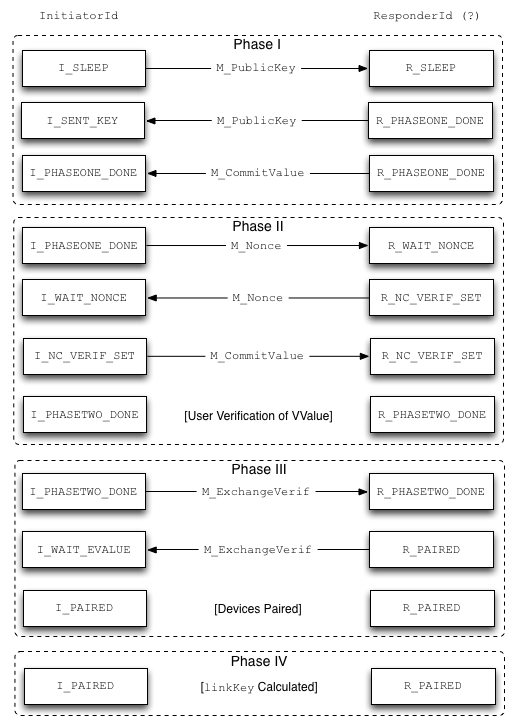
\includegraphics[width=0.8\textwidth]{diagrams/transitions.png}
        \caption{A diagram describing the transitions of the initiator and responder, and the messages that are passed across during SSP. Created by the author.}
        \label{transitions}
    \end{center}
\end{figure*}

\begin{figure*}
    \begin{center}
        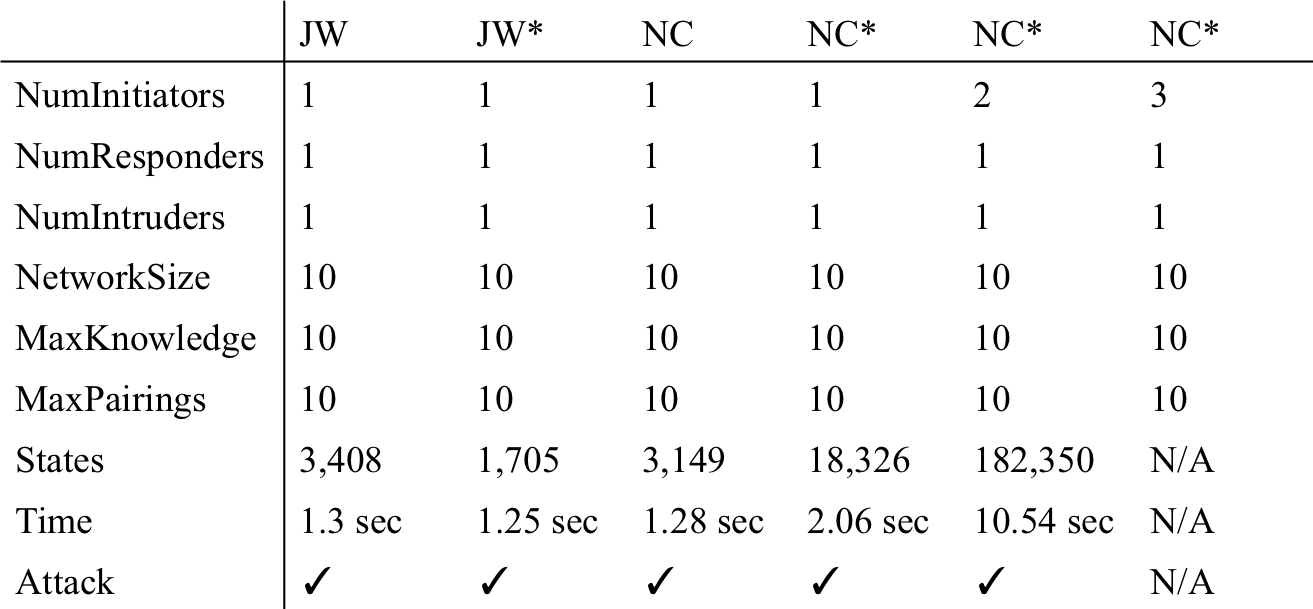
\includegraphics[width=0.8\textwidth]{diagrams/state_table.png}
        \caption{Table of Murphi state exploration results when searching for attacks. Created by the author. * denote the models that are tested when the intiator cannot initiate a connection with an intruder device.}
        \label{state_table}
    \end{center}
\end{figure*}

\begin{figure*}
    \begin{center}
        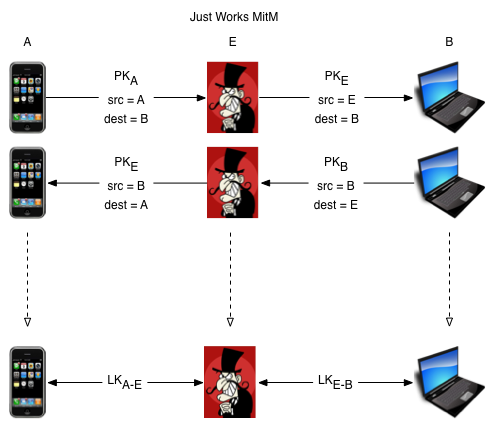
\includegraphics[width=0.8\textwidth]{diagrams/jw_mitm.png}
        \caption{A diagram describing the MitM attack for the Just Works association model. Created by the author.}
        \label{jw_mitm}
    \end{center}
\end{figure*}

\begin{figure*}
    \begin{center}
        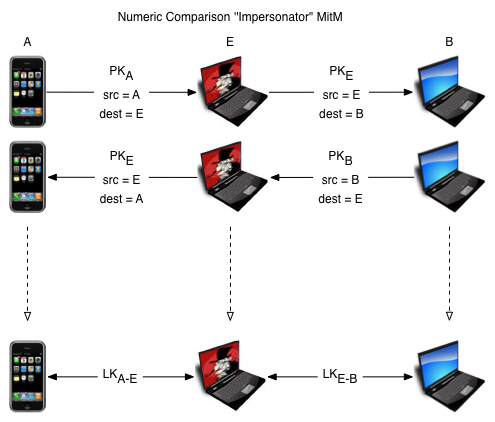
\includegraphics[width=0.8\textwidth]{diagrams/nc_impersonator_mitm.png}
        \caption{A diagram describing the ``impersonator'' MitM attack for the Numeric Comparison association model. Created by the author.}
        \label{nc_impersonator_mitm}
    \end{center}
\end{figure*}

\begin{figure*}
    \begin{center}
        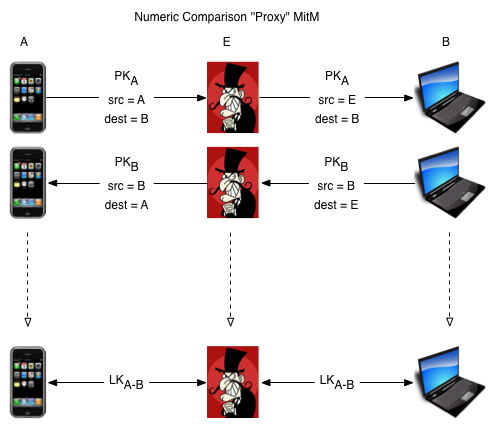
\includegraphics[width=0.8\textwidth]{diagrams/nc_proxy_mitm.png}
        \caption{A diagram describing the ``proxy'' MitM attack for the Numeric Comparison association model. Created by the author.}
        \label{nc_proxy_mitm}
    \end{center}
\end{figure*}

\balancecolumns
\end{document}
 